\documentclass[border=10pt]{standalone}

\usepackage{tikz}
\usepackage{tikzsymbols}
\usetikzlibrary{calc,patterns,shapes.geometric}

\def\centerarc[#1](#2)(#3:#4:#5){\draw[#1] ($(#2)+({#5*cos(#3)},{#5*sin(#3)})$) arc (#3:#4:#5);}

\begin{document}
	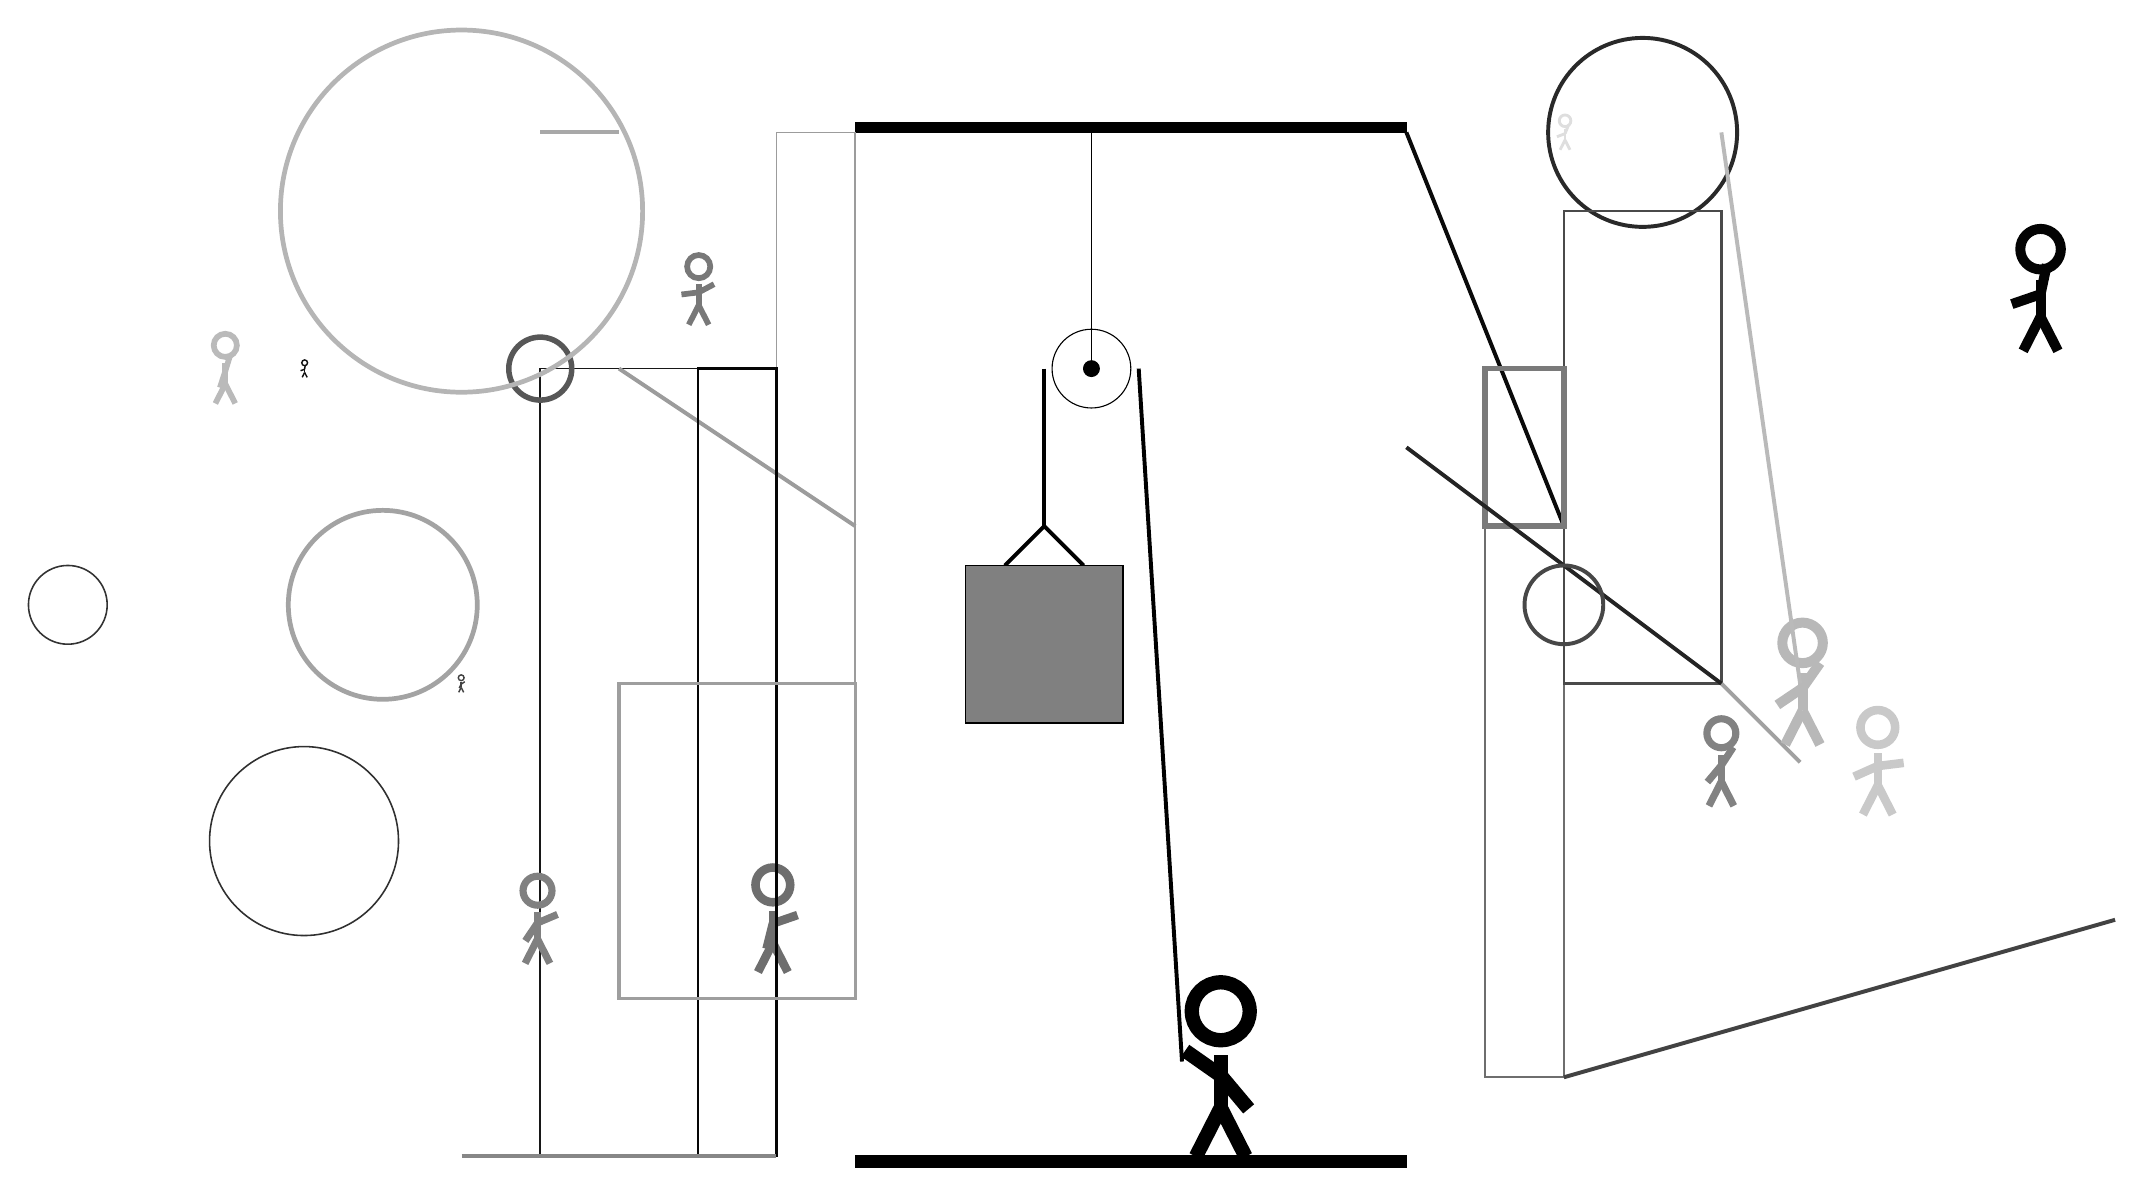
\begin{tikzpicture}
		%%%%% START %%%%%
		
		\draw[fill=black] (-2, 10) rectangle (5, 10.125);
		
		\draw (1, 7) circle (0.5);
		\draw[fill=black] (1, 7) circle (0.1);
		\draw (1, 10) -- (1, 7);
		
		\node[line width=0.4mm, color=black!57] at (-3, 0) {\Strichmaxerl[6][76][19]};
		
		\node[line width=0.4mm, color=black!49] at (9, 2) {\Strichmaxerl[5][50][57]};
		\draw[line width=0.2mm, color=black!91] (-4, -3) rectangle (-6, 7);
		\draw[line width=0.5mm, color=black!34](-5, 10) -- (-6, 10);
		\draw[line width=0.2mm, color=black!39] (-3, -1) rectangle (-2, 10);
		\draw [line width=0.5mm, color=black!84](8, 10) circle (1.2);
		\draw[line width=0.3mm, color=black!57] (6, 7) rectangle (7, -2);
		
		\draw [line width=0.2mm, color=black!81](-9, 1) circle (1.2);
		\draw[line width=0.3mm, color=black!71] (7, 3) rectangle (9, 9);
		
		\draw [line width=0.7mm, color=black!66](-6, 7) circle (0.4);
		
		\draw[line width=0.5mm, color=black!39](-2, 5) -- (-5, 7);
		\node[line width=0.4mm, color=black!27] at (-10, 7) {\Strichmaxerl[4][72][73]};
		\node[line width=0.4mm, color=black!13] at (7, 10) {\Strichmaxerl[2][21][68]};
		\draw [line width=0.2mm, color=black!80](-12, 4) circle (0.5);
		\draw[line width=0.5mm, color=black!37](9, 3) -- (10, 2);
		\draw[line width=0.5mm, color=black!96](7, 5) -- (5, 10);
		
		\draw[line width=0.7mm, color=black!52] (6, 5) rectangle (7, 7);
		\draw [line width=0.6mm, color=black!36](-8, 4) circle (1.2);
		\draw[line width=0.3mm, color=black!98] (-3, -3) rectangle (-4, 7);
		\draw [line width=0.6mm, color=black!29](-7, 9) circle (2.3);
		\node[line width=0.3mm, color=black!28] at (10, 3) {\Strichmaxerl[7][34][55]};
		
		\draw[line width=0.5mm, color=black!47](-7, -3) -- (-3, -3);
		\draw[line width=0.4mm, color=black!38] (-2, -1) rectangle (-5, 3);
		\node[line width=0.5mm, color=black!99] at (13, 8) {\Strichmaxerl[7][19][78]};
		\node[line width=0.6mm, color=black!94] at (-9, 7) {\Strichmaxerl[1][20][82]};
		
		\draw[line width=0.5mm, color=black!74](7, -2) -- (14, 0);
		\node[line width=0.3mm, color=black!50] at (-6, 0) {\Strichmaxerl[5][56][23]};
		\draw[line width=0.5mm, color=black!27](9, 10) -- (10, 3);
		
		\draw[line width=0.5mm, color=black!86](9, 3) -- (5, 6);
		\node[line width=0.5mm, color=black!21] at (11, 2) {\Strichmaxerl[6][24][7]};
		\node[line width=0.7mm, color=black!74] at (-7, 3) {\Strichmaxerl[1][62][35]};
		
		\node[line width=0.4mm, color=black!53] at (-4, 8) {\Strichmaxerl[4][7][28]};
		\draw [line width=0.5mm, color=black!72](7, 4) circle (0.5);
		
		\draw[line width=0.5mm] (-0.1, 4.5) -- (0.4, 5.0) -- (0.9, 4.5);
		\draw[fill=black!50] (-0.6, 4.5) rectangle (1.4, 2.5);
		
		\draw[line width=0.5mm] (0.4, 7) -- (0.4, 5.0);
		\centerarc[line width=0.5mm](1, 7)(0:180:0.6);
		\draw[line width=0.5mm](1.6, 7) -- (2.15, -1.8);
		
		\node at (2.6, -1.9) {\Strichmaxerl[10][-35][-50]};
		
		\draw[fill=black] (-2, -3) rectangle (5, -3.15);
		
		%%%%% END %%%%%
	\end{tikzpicture}
\end{document}